\chapter{Conclusion}

\section{Future Work}

Of the two implementations, the obstruction detector appears to be the better candidate for further development. 

\subsection{Further Assessment and Improvements of the Obstruction Detector}

Some topics that should be considered:

\begin{description}

\item[- Lighting conditions] The system should be tested in many different lighting conditions. It is of interest to investigate: Different light sources: sunlight, light armatures, lightbulbs, LED, etc.; Direction of incoming light, how shadows and reflections can fool the system. This analysis can be quantitative. 

\item[- Negative Obstacles] A hole in the ground or a downwards staircase are examples of negative obstacles. Such obstacles can be perceived with the current configuration if the disparity map is dense enough. A hole in the ground could be detected with a dense disparity map, and an accurate floor filter. Then the hole will be detected as a dark gray area on a black (zero intensity)  background.

\item[- How Different Surfaces Influence Matching] Revealing how reflective or transparent surfaces will influence the stereo matching is important in order to increase the robustness of the system.

\item[- A Working Floor Filter] This is a key critical in the current implementation.

\end{description}

\begin{wrapfigure}{r}{0.55\textwidth}
	\vspace{-10pt} % Remove exessive whitespace
	\centering
	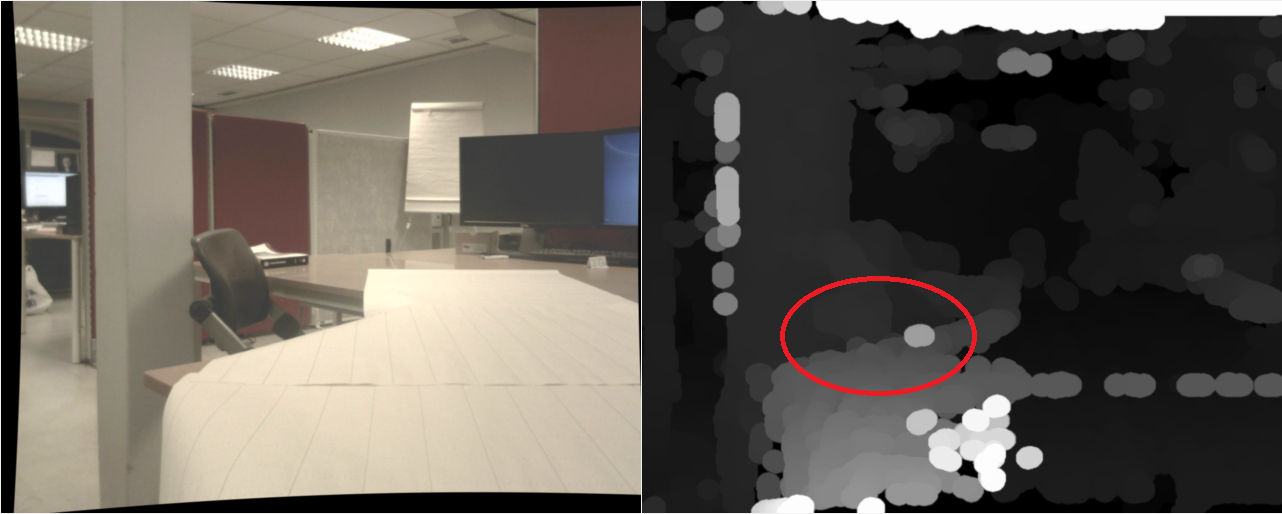
\includegraphics[width=0.52\textwidth]{pitfall_concept_highlighted}
	\caption{\label{fig:pitfall} Example of a negative obstacle. The disparities have been dilated to give the appearance of a denser disparity map.}
	%\vspace{-20pt} % Remove exessive whitespace
\end{wrapfigure}



\subsection{Integration With Point Cloud Library (PCL)}

A great deal of time was spent on an attempt to integrate Qt and OpenCV with the Point Cloud Library (PCL). Needless to say, the integration was not successful. PCL is an open source project for image and point cloud processing \cite{pcl}. Similarly to OpenCV, it is free of charge, and the source code is available for download on the project home page and on GitHub. PCL depends on many 3rd party libraries which must be downloaded and compiled separately. This complicated the integration process, and was the most significant hindrance to a successful integration.



\subsection{New Hardware}

\paragraph{Visual Sensors}

The current camera set-up comes with limitations that makes them unsuitable as navigational sensors. The video feed is unsynchronized, which makes the disparity map useless whenever there is relative motion between the cameras and the surroundings. 

\paragraph{Computing Hardware Suitable for Image Processing} At the moment, all image processing is done on a remote computer because of several reasons. The  computer on the robot had very limited storage, limited computational power. \gls{opencv} is a large library which requires several gigabytes of storage. In addition, processing can potentially be speeded up significantly by hardware acceleration with a \gls{gpu}. A drawback is increased power consumption and reduced range.

\subsection{Additional Functionality}

\paragraph{Visual Servoing of Robotic Arms}

Visual control of robotic arms can be an additional task for a sensor already used for mobility control. There are two common sensor configurations: eye-in-hand, where the camera is on the manipulator; eye-to-hand, where the manipulator is observed from a distance. Some drawbacks with visual servoing, is that the robot is constrained to  the cameras field of view, and that line of sight between camera and robot can be obstructed.

Visual sensors have been used in safe human-robot collaboration where the robot will sense and adapt to proximity by slowing down or by dynamically planning a different path\cite{sintefKinect}.

\section{Task Fulfilment}
 
\subsection{Point 1 - Find Methods}
Chapter \ref{chp:theory} introduced several applications of computer vision that could be used in vehicle navigation. Stereo vision was one of the main topics within the chapter. \gls{slam} based on computer vision was mentioned as way to create dense three dimensional maps based on a depth sensor. 

It was understood in an early phase of the project that the scope of autonomous navigation is huge. An extensive treatment of the major aspects in autonomous navigation was considered to be a unrealistic goal. Therefore, the report scope had to be limited. Because of this, the theme in this report became more geared towards the sensing part of navigation. 
 
\subsection{Point 2 - Implementation}
An obstruction detector based on stereo vision and a vanishing point detector was implemented during the project period. No new equipment was installed, except for the camera bracket for the new camera position.  
 
\subsection{Point 3 -  Performance and Suitability}

An assessment of the implementation is presented in chapter \ref{chp:conclusion}. 
 
\subsection{Point 4 - Handling of Errors and Hazards}
The implementations themselves can be considered to be proofs-of-concept, rather than development projects. Their purpose is to demonstrate a technology. Some safety and reliability aspects are discussed in chapter \ref{chp:assessment}.
  
\subsection{Point 5 - Changes and Further work}
The section on future work comes with several suggestions for further testing and expansions, which may increase robustness. 

\section{Final Conclusion}

An application written in C++, using \textit{Qt 5.5} and OpenCV (Open Source Computer Vision Library), is able to form a depth map based on two rectified input images. It has been shown how two IP camera can be combined to form a stereo camera, which serves as video input to the application. The cameras were calibrated, both separately and in stereo, in order to make stereo matching possible. Stereo matching yielded dense disparity maps when applied to still sample images (e.g. Tsukuba). When live camera feed from the IP cameras was provided as input, the resulting disparity map was significantly more noisy and much less dense. 

The computed disparity image can be used to detect obstacles in the path of the robot. The detector is able to detect objects between at least 38 cm, and up to an upper limit of 2 - 3 meters. The upper limit can be set in the program source code. 